\chapter{Introduction}\label{ch_intro}
\chapterauthor{Jeff Yoshimi}

% Change most italics to glossary items
% Consider changing some of the Simbrain pictures so that the size of the weights is more evident, since that is now discussed
% Maybe use some of the blue brain / human brain project pics. They are amazing.
% Need terminology for input and output to a specific weight layer. Comes up in backprop for example

% Sometimes "network" in biology also refers to networks of _brain areas_. See ch. 3
The phrase ``neural network'' has several meanings. A \glossary{biological neural network} is an actual set of interconnected neurons in an animal brain. Fig. \ref{introNets} (left) shows a biological neural network. ``Neural network'' can also mean \glossary{artificial neural network} (or ``ANN"),  that is, a computer model that has certain things in common with biological neural networks. Fig. \ref{introNets} (right) shows an artificial neural network. It has ``nodes'' and ``weights'' that are analogous to the neurons and synapses of a biological neural network. We focus on artificial neural networks in this book, and when we refer to ``neural networks'' we usually mean artificial neural networks.
% There are other ways referring to artificial neural networks, including: ``connectionist network,' or' ``PDP (parallel distributed processing) network. These differ slightly but will be treated as synonyms in what follows.

\begin{figure}[h]
\centering
\raisebox{-0.5\height}{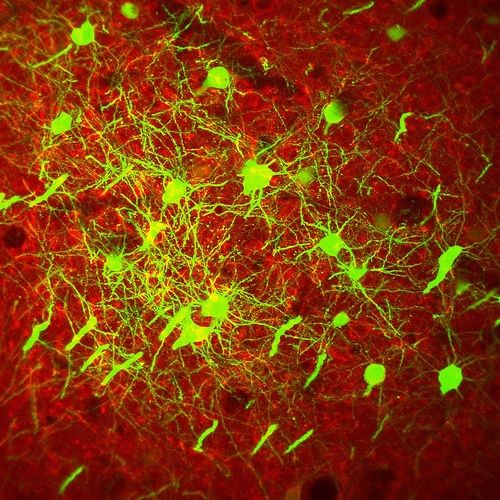
\includegraphics[scale=.3]{./images/NeuroNet.jpg}}
\hspace*{.2in}
\raisebox{-0.5\height}{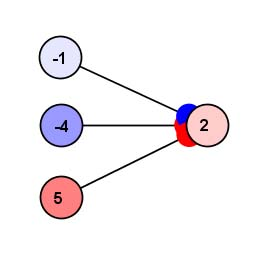
\includegraphics[scale=.5]{./images/Simple3.jpg}}
\caption[Left: Mark Miller, Nelson Lab, Brandeis University. Licensed Under: CC BY-ND; Right: Simbrain screenshot.]{Left: A biological neural network. Right: A simple artificial neural network built in Simbrain, with three nodes connecting to another node via three weights.}
\label{introNets}
\end{figure}

Neural networks can be made to do many fascinating things. They can, for example, drive cars, forecast weather patterns, recognize faces in images, and play the game Go at championship levels. In the early 2020s the emergence of ``generative AI'' (see section \extref{age_generative_ai}) based on neural networks revolutionized the field, and they have since become a pervasive feature of human life. (For better or worse? The debate is far from settled!) They speak language fluently, and produce realistic text, audio and video, often within seconds. They have been used to model the brain at all of its levels, from individual neurons up to the entire brain. They have been used to model cognition in all of its forms, including memory, perception, categorization, language, and attention. In this chapter, we give a general introduction to neural networks, and survey some of these different ways they are used.\footnote{Some time in the 2010s or 2020s, it became standard to refer to neural networks as a form of ``AI'' or "Artificial Intelligence.''  From this standpoint, ``AI'' is a covering term that includes all the many forms of computer simulation that attempt to behave in an intelligent and often human-like manner.  In the earlier literature ``AI'' was used to refer to more classical, symbolic forms of artificially intelligent system, and in that era there was a kind of battle between AI and neural networks. Some of this history is covered in section \extref{cog_rev}.  The term ``AI'' is mostly avoided in this text.}

\section{Structure of Neural Networks}\label{structureNets}

In figure \ref{nodesWeights} a simple neural network is shown with some of its parts labeled. In this section, we review the parts of neural networks (nodes and weights), the ways they can be structured (their topology), and the relationship between a network and its environment. In each case, bear in mind that what precisely the concepts mean depends on the type of model we are dealing with.\footnote{Neural networks can be used for engineering, modeling the brain, or modeling the mind. These different uses are discussed in chapter \ref{ch_applications}. Depending on the way a network is being used, the way its parts are interpreted differs, as we'll see.} 

\begin{figure}[h]
\centering
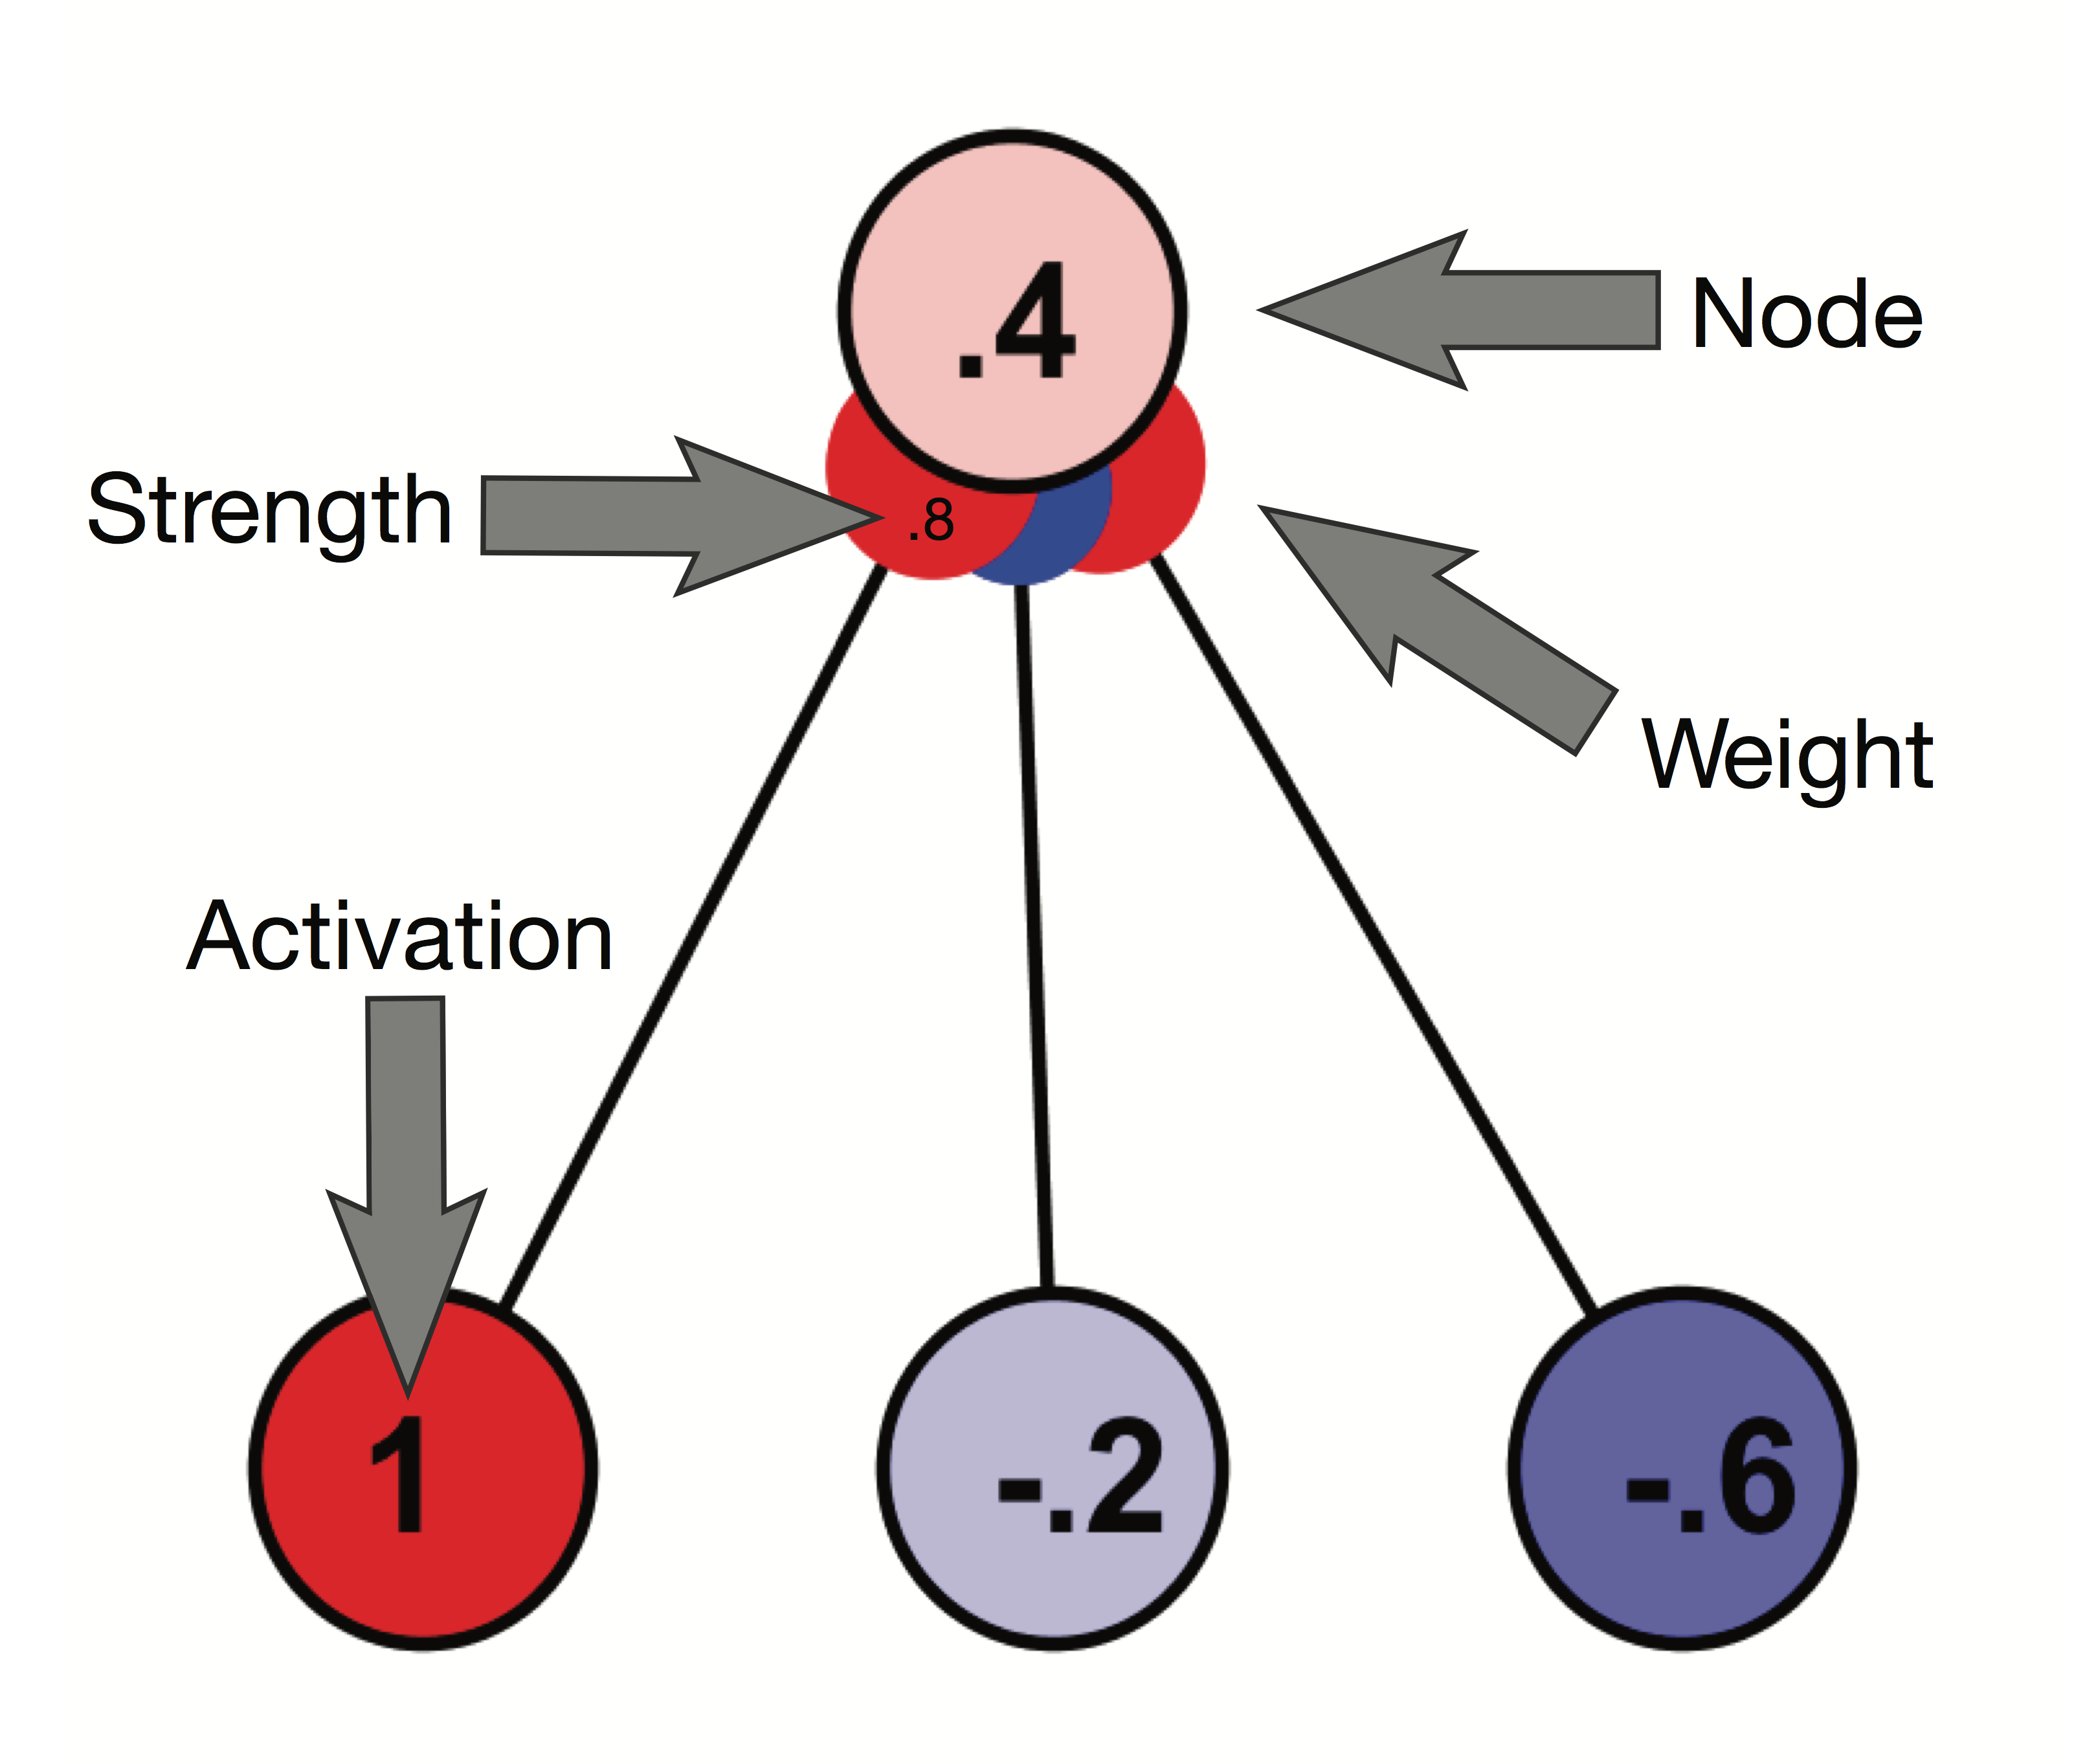
\includegraphics[scale=.2]{./images/labelledNet.png}
\caption[Simbrain screenshot with additional elements added by Pamela Payne.]{Nodes and their activations; weights and their strengths.}
\label{nodesWeights}
\end{figure}

In the figure, a circle with a number in it is an artificial neuron or \glossary{node} (nodes are also referred to as ``units'').\footnote{Sometimes, when the context makes it clear that we are talking about an artificial neural network, terms like ``neuron'' and ``synapse'' are used to mean artificial neuron (node) or artificial synapse (weight).}  The number inside a circle corresponds to that node's \glossary{activation}. In Simbrain, red corresponds to an ``active'' neuron (activation greater than 0), and how deep the red is corresponds to how close the activation is to its maximum value. Blue corresponds to an ``inhibited'' neuron (activation less than 0), and how deep the blue is corresponds to how close the activation is to its minimum value. White corresponds to an inactive neuron (activation equals 0). In a computational neuroscience model, these activations might represent the firing rate or membrane potential of a real neuron. In a psychological model, the number might represent the presence of an item in working memory, or the strength of an unconscious belief. As we will see, there is a great deal of variance in what concepts such as activation are taken to mean.
%In computational neuroscience, the numbers represent real properties of neurons and synapses. For example, in some models activation represents a firing rate (number of spikes per second), and in other models it represents a voltage. Weight strength in such models represents the efficacy of a synapse in transmitting information from one neuron to another. In connectionist models of psychological data, the interpretation of activation and weight strength is more abstract. Node activations are sometimes taken to represent the overall activity of a whole population of neurons in some region of the brain, something abstract like the ``strength of a hypothesis'', and they are sometimes simply taken to be hidden variables that have no biological significance whatsoever. \footnote{As McCLelland, Rummelhart, and Hinton put it: ``These models assume that information processing takes place through the interactions of a large number of simple processing elements called units, each sending excitatory and inhibitory signals to other units. In some cases, the units stand for possible hypotheses about such things as the letters in a particular display or the syntactic roles of the words in a particular sentence. In these cases, the activations stand roughly for the strengths associated with the different possible hypotheses, and the interconnections among the units stand for the constraints the system knows to exist between the hypotheses. In other cases the units stand for possible goals and actions... and the connections relate goals to subgoals, subgoals to actions, and actions to muscle movements. In still other cases, units stand not for particular hypotheses or goals, but for aspects of these things'' \cite{mcclelland1986appeal}. Or again, as Sejnowski and Rosenberg say: ``The processing units in a network model share some of the properties of real neurons, but they need not be identified with processing at the level of single neurons. For example, a processing unit might be identified with a group of neurons, such as a column of neurons'' (Sejnowski and Rosenberg, p. 146) \cite{sejnowski1987parallel}.}
%  From Cohen et. al on Fear: "Processing units: Simple, nonlinear summing devices can be used as a first approximation of the behavior of populations of real neurons that redundantly code for the same piece of information."
% Perhaps the best discussion of this issues is in Smolensky PTC. (Around table 1)

The lines with filled disks at the end of them are artificial synaptic connections or \glossary{weight}s. These correspond to connections between nodes, which control how activation flows through a network. The weights have a value, a \glossary{strength}. The larger the absolute value of a weight strength, the ``stronger'' it is.  2 is a stronger positive weight than 1 is, and -2 is a stronger negative weight than -1 is. Thus, to strengthen a weight is to increase its absolute value, and to weaken it is to reduce its absolute value.  Stronger weights are shown as larger disks in Simbrain. The actual weight strength can be seen by hovering over the weights or double clicking on them.  As activation flows through a network, the weights with a positive strength (the red weights in Simbrain) tend to enhance activation, and the weights with a negative strength (the blue weights) tend to reduce activation.\footnote{For more details on the graphic representation see \url{http://www.simbrain.net/Documentation/v3/Pages/Network/visualConventions.html}.} In neuroscience terms, these correspond to excitatory and inhibitory synapses (and the neurons at the source of these synapses called excitatory and inhibitory neurons). As you play with simulations in Simbrain and study the chapters to come, you will begin to get a feel for how different kinds of weights have different kinds of impacts on the flow of activation in a network. 

What weight strength represents depends on what kind of model we are dealing with (see chapter \ref{ch_applications}). In a computational neuroscience model, it would represent \glossary{synaptic efficacy}--roughly speaking the impact a pre-synaptic neuron can have on a post-synaptic neuron after the pre-synaptic neuron fires an action potential. In a connectionist or psychological model, the strength might represent an association between concepts. In a machine learning model, there might be no direct interpretation of weight strengths at all: they are mere parameters in a statistical model that does something useful, like recognize faces in images.

Node activations change in accordance with \emph{activation functions} (discussed in chapter \extref{ch_act_functions}), and weight strengths change in accordance with different types of learning algorithms discussed throughout the book. Indeed, how to train neural networks is one of the most fundamental topics in the field, and is the focus of several chapters, including chapters \extref{ch_unsupervised}, \extref{ch_supervised} and \extref{ch_lms_backprop}. 

In some models, a node can also produce a \glossary{spike}, which is a discrete event that corresponds to the action potential of a neuron.\footnote{A spike is represented in Simbrain by a node and all its outgoing connections turning yellow. For an illustration of a spiking node and how it looks in Simbrain, see \url{http://www.simbrain.net/Documentation/v3/Pages/Network/neuron.html}.}  Spiking neurons have their own rules and structures, which we discuss in chapter \extref{ch_spiking}.

Nodes and weights are the basic parts of a neural network. Together, they form a network structure, or mathematically, a graph\footnote{\url{https://en.wikipedia.org/wiki/Graph_(discrete_mathematics)}.}, where the nodes correspond to vertices, and the weights correspond to edges.\footnote{A neural network is a special type of graph: a vertex-labeled, edge-labeled, directed graph. This means that the edges between nodes have a direction (the graph is \emph{directed}), and that numbers are associated with the vertices and edges (it is \emph{vertex-labeled} and \emph{edge-labeled}).}  The graph-structure formed by a network's nodes and weights is the network's \glossary{topology}. At a first pass, neural network topologies fall into one of two rough types shown in Fig. \ref{nn_types}: feed-forward and recurrent. 

% Another issue with layer concept. Sometimes it refers just to activations, sometimes to activations and all the hyperparameters, rules, etc. (i.e. what would show up in a property editor if you double clicked.)
% Are pools of IAC node layers?
% See deep leaning chapter and convolutional layers and cohere with that. Feature maps are a kind of node layer (a tensor) and convolutional layers are a special kind of weight layer.
A  \glossary{feed-forward network} is a sequence of \emph{layers} of unconnected neurons stacked on top of each other such that each layer is fully connected to the next one in the sequence (each node in one layer sends a connection to every node in the next layer).\footnote{\label{acyclic} In graph-theoretic terms, such a network is a directed, acyclic, multipartite graph. It is is \emph{acyclic} because there are no \emph{cycles}; there is is no way to ``move'' from one vertex back to itself along a sequence of vertices connected by edges. It is \emph{multi-partite} because the vertices can be partitioned into \emph{independent sets} (node layers), within which none of the vertices are connected. When such a network is not fully-connected from one layer to the next, it is still often referred to as ``feed-forward''. In some cases a \glossary{skip connection} bypasses a layer (for example, going straight from input to output despite the presence of a hidden layer). Since activity still flows ``forward'', this will be referred to as a feed-forward network.}  Activity in this kind of network flows from an \emph{input layer} through a sequence of \emph{hidden layers} and then to an \emph{output layer}. Sometimes there are no hidden layers and we have a feed-forward network that connects directly from an input layer to an output layer.
% The hidden layer is often the key. It's what takes from behaviorism to cog-sci with internal reps. It's a latent space. It's where the internal reps are.

% TODO: Forward references
 In a feed-forward network activity simply passes through the node layers; when activation is added to the input nodes and the network is updated, that activation flows from layer to layer and is then erased. Feed-forward networks are often classifiers: an input (which might represent an image, or a smell) passes through the layers of the network, and the output activations then represent a way of classifying the input (saying who is in the image, or what object is being smelled).

% Also a link to overfitting?
In a feed-forward network we can distinguish between a \glossary{node layer} and a \glossary{weight layer}.\footnote{The distinctions introduced in this paragraph and the next one are stipulations made to organize the material in a coherent way. Terms like ``node layer'' and ``weight layer'' are not standard, but they help organize the material in this book.} We will take node layers in a feedforward network to be collections of nodes that are treated as a group, and weight layers to be collections of weights that connect node layers. Often, node layers are represented using vectors and weight layers using matrices (see chapter \extref{ch_linear_algebra}). The network in Fig. \ref{nn_types} has three node layers (labelled ``input layer'', ``hidden layer'', and ``output layer'') and two weight layers (labelled ``1-2'' and ``2-3'').\footnote{To make matters even more confusing, sometimes the input node layer is \emph{not} counted as a layer.} When used without qualification, we use the term ``layer'' to mean ``node layer''.\footnote{In Simbrain, node and weight layers are both represented as groups, indicated by the yellow interaction boxes: \url{http://www.simbrain.net/Documentation/v3/Pages/Network/groups.html}.}

% Add link to universal approximator thing once we have it
We can also distinguish between the ``representational depth'' and ``representational width'' of a feed-forward network.  We take the \glossary{representational depth} of network to correspond to how many layers or layer-like structures the network has. Thus a ``deep'' network is one with many node and weight layers. The \glossary{representational width} of a given node layer corresponds to how many nodes it has.\footnote{While the concept of depth is fairly common, ``width'' as a named concept is not. Be aware that ``width'' and ``depth'' are also used to refer to the shapes of tensors (see section \extref{sect_tensors}), but the meaning is different there, and we assume our meaning is clear in context.} We will see throughout the book that these two concepts provide distinct ways of understanding the representational capacities of neural networks. A wider layer can develop more sophisticated representations of its inputs. A network with more depth can develop representations that combine features of other representations, so that we get increasingly complex ``representations of representations.'' The layers of a network trained to recognize images can go from representing lines, to sets of lines (that is, shapes), to sets of shapes, etc. (see the discussion of Selfridge in chapter \extref{ch_history}, and of convolutional networks in chapter \extref{ch_cnn}). Analogues of these intuitive concepts of depth and width persist in more complex types of networks, like transformers (chapter \extref{ch_transformers}), where we can contrast the number of heads in a given block (width) with the number of blocks that are stacked on top of each other (depth). 
 
\begin{figure}[h]
\centering
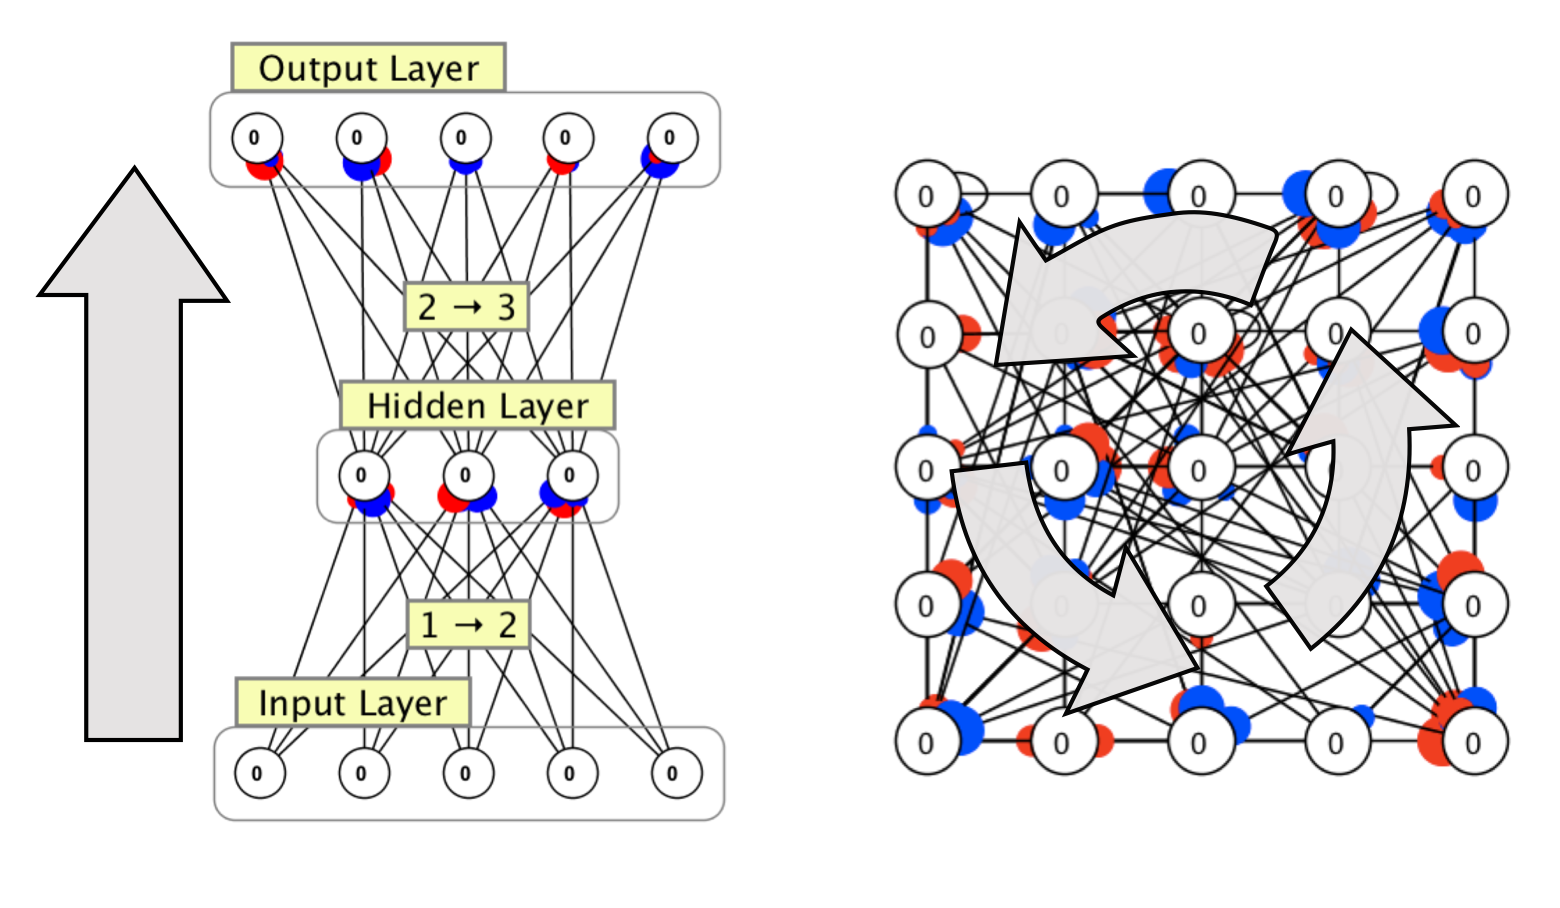
\includegraphics[scale=.7]{./images/NeuralNetTypes.png}
\caption[Simbrain screenshots with additional elements added by Pamela Payne.]{Feed-forward network (left) and recurrent network (right). Gray arrows give a sense of how activation flows through them. The feed--forward network has 3 node layers (a representational ``depth'' of 3, which is not deep; this is not a ``deep network''), and the layers have representational ``widths'' of 5, 3, and 5. }
\label{nn_types}
\end{figure}

%The effects of any input to the network on the network will be completely erased after $n$ iterations where $n$ is the number of layers.
% The graph representing weights from one layer to layer to the next in a feed-forward network is an example of a bipartite graph.

In a \glossary{recurrent network}, the nodes are interconnected in such a way that activity can flow in repeating cycles.\footnote{In graph-theoretic terms, this is a cyclic graph, which contains at least one cycle. Recall from footnote \ref{acyclic} that a directed cycle is a sequence of directed edges that begin and end at the same vertex. That is, starting at one node of such a network, we can ``travel'' from one node to another via the connections and end up back where we started.} Recurrent networks display complex dynamical behaviors that don't occur in feed-forward networks since activity in the network cannot always ``leave'' the network. Most biological neural networks are recurrent. In machine learning, recurrent networks can be used to simulate dynamical processes, for example,  to mimic human speech, or create artificial music.
% Forward ref to DST for a way to study and visualize these
% Any input to such a network \emph{influences} rather than dictates the network's future states, which are determined by both the current input and the current state of the network (itself a product of previous inputs and/or the network's own internal dynamics). 

\begin{figure}[h]
\centering
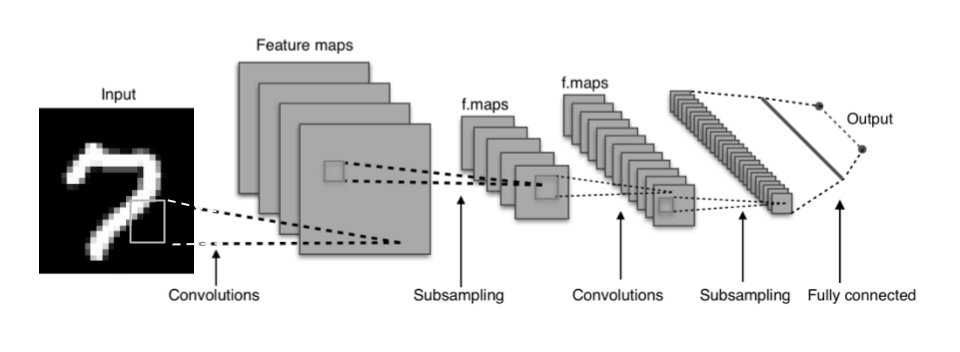
\includegraphics[scale=.45]{./images/deepNet.png}
\caption[Adapted from a creative commons image by Aphex34 at \url{https://commons.wikimedia.org/wiki/File:Typical_cnn.png} ]{A deep neural network, trained to recognize images. The convolutional layers scan over the inputs they are linked to. Note that individual nodes and connections are not visible in this image.}
\label{deep_net}
\end{figure}

% Tensor glossary entry. By convention tensor is rank 3 (or more? and used for nodes. Check this. Each sub matrix is  features maps.  
% Each convolutional layer is associated with a fixed set  of weights that is shared. These do different things. Their results are added together. TODO: Fix the picture so it is clear that each 2d node array in each node tensor is associated with a separate convolutional weight layer, which scans across the input.

% History ref
The distinction between feedforward and recurrent networks is a useful first-pass way to organize the field. However, more complex architectures are possible, and since the 2010s, two specific architectures have been especially common: convolutional networks and transformers.  There is not space to go into these structures here, but we discuss them in chapters \extref{ch_cnn} and \extref{ch_transformers}. These networks operate on data structures more complex than arrays of numbers, for example on 3d arrays or volumes of numbers, which are a kind of tensor (tensors are discussed in section \extref{sect_tensors}). An example of a convolutional network is shown in figure \ref{deep_net}. Networks like this are so large that we can't represent each node and weight separately, and the concept of a layer becomes more complex as more structure and processing is packed into each layer. But the basic concepts of feedforward and recurrent networks that structure the first part of this book still are useful for understanding these more complex forms of neural network. 

\begin{figure}[h]
\centering
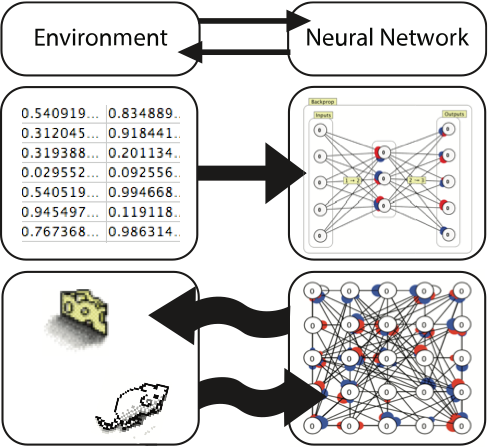
\includegraphics[scale=.7]{./images/nn_environment.png}
\caption[Pamela Payne.]{The relationship between a neural network and an environment. An ``environment'' is often something as simple as a table of values (middle row). However it can also be something more complex, like a virtual world (bottom row).}
\label{nn_environment}
\end{figure}

% Forward ref on RL
Networks almost always exist in some kind of  \glossary{environment}, which gathers inputs for a network and receives its outputs. In cognitive science, the environment of our brain's neural network is the literal environment around us. In some simulations--for example, reinforcement learning simulations--simulated environments are used for neural networks. But if we take environment in a broader sense to simply be whatever it is that produces inputs to an artificial neural network and whatever deals with the outputs, then we capture a broader range of cases.\footnote{Here again we are using ``environment'' in a technical sense that does not track all standard usage, but that is useful for organizing the material and that also draws helpful conceptual connections.}  For example, a neural network that converts speech to text can be connected to audio sensors, like the microphone on your phone. It can take audio in, convert it to text, and send the result out via the speakers. By far the most common way a neural network is linked to inputs and outputs, especially when building and testing them, is via tables of data. Training and testing datasets are discussed at length in chapter \extref{ch_data_science}. In Simbrain, we will also link neural networks to virtual environments. Figure \ref{nn_environment} shows how some of these configurations might look. Couplings between a network and an environment occur at special nodes:  an \glossary{input node}  is influenced by the environment, while an  \glossary{output node} exerts an influence on the environment. In figure \ref{nn_types} (left), for example, the input nodes are the nodes in the input layer, and the output nodes are the nodes in the output layer.\footnote{Information on how to couple nodes to an environment in a Simbrain simulation, and thus treat them as input or output nodes, is available here: \url{http://www.simbrain.net/Documentation/v3/Pages/Workspace/Couplings.html}.} 
%The recurrent network on the right might also have input and output nodes (or nodes that are both at once), but this is not directly visible in that figure.

\section{Computation in Neural Networks}\label{intro_comp_nn}

We've seen what the parts of a neural network are and learned some basic concepts relating to their structure. We now consider  how computation works in neural networks. We first develop a basic intuition for how they channel information, and then consider how they are trained (rather than being programmed), and contrast all this with computation in a standard computer.

\subsection{Performance vs. Learning}\label{performanceLearning}

% Forward reference to in-context learning as another approach
% See Smolensky distinction between activation evolution equation and connection evolution equation. Footnote. Use that in DST too and refer back.  
% Cohere this with the first demo.  Split into input adjustment and weight adjustment and two cases for each. (1) strengthen excitatory input -> increase output.  (2) strength inhibitory input -> decrease output. ...  Tap up > space > up > space to see what happens. (3) strengthen excitatory weight > increase output   (4) strengthen inhibitory weight > decrease otuput. Notice how by adjusting up and down you can get what you want 

To develop an intuition for how neural networks ``channel information'' we can break the issue into two parts: performance and learning. \glossary{Performance} (or \glossary{inference}) corresponds to how activations flow through a network, given a fixed pattern of connectivity.\footnote{As of 2025 the term ``inference'' has become more common. The term ``performance'' derives in part from psychology, where it refers to behavioral performance, like performance on a task.  An issue with the term (especially in engineering) is that it also describes how \emph{well} a neural network does at some task. The term ``inference'' derives from statistics, where one might refer to statistical inference with a trained model. An issue with the term is that it is also suggestive of logical inference, which is not the right connotation for a neural network. So each term has its pros and cons.}  \glossary{Learning} corresponds to how patterns of connectivity (and other networks parameters) are adjusted, usually in an effort to make a neural network perform more effectively. These are two different types of dynamics--a fast dynamics of performance and a slower dynamics of learning--and it is important to get a feel for them right from the start.
 
To understand how performance works, we consider a network that has already been trained, and ask how different inputs propagate through it. That is, we don't change its weights but only change its inputs to see how it responds, given its weights. When you use ChatGPT, you are using a network whose weights have already been set. You are using the final product of a long training process. You write text prompts, they are converted to activations, these propagate through a bunch of nodes, and new text is generated as a result, one token at a time.  When you talk to a grown person, something similar is happening. They are not learning (much) over the course of a few seconds, but neurons are firing in the brains and their internal networks are reacting to what you say.  

\begin{figure}[h]
\centering
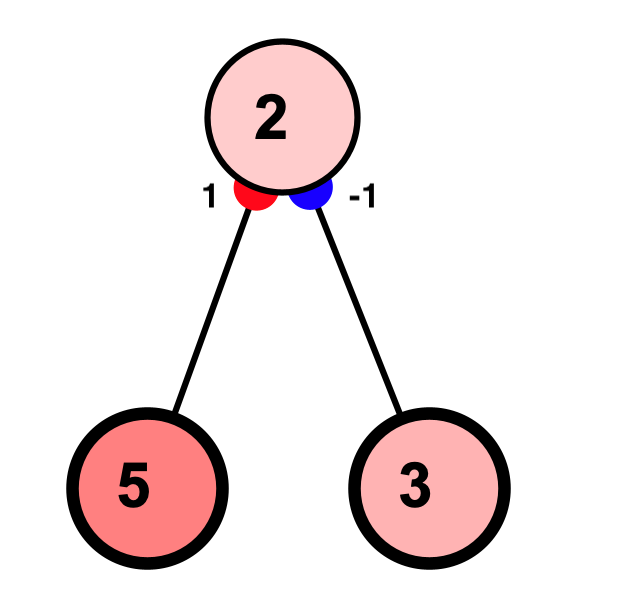
\includegraphics[scale=.5]{./images/2NodeSimpleFF.png}
\caption[Simbrain screenshot.]{A simple feed-forward network with clamped inputs, which can be used to develop an intuition for how performance and learning work. The nodes are linear nodes that take a weighted sum of inputs. The weight strengths are $1$ and $-1$, so the output is $5 \times 1 + 3 \times -1 = 5 - 3 = 2$. By adjusting the inputs up and down, we can make the output activation be whatever we want within the upper and lower bounds of a node (performance). Or, for a fixed pattern of input, we can make the output be whatever we want it to be by changing the weights.}
\label{2NodeSimpleFF}
\end{figure}

How does this work? Consider the network shown in figure \ref{2NodeSimpleFF}: it's a simple feed-forward network with two input nodes and one output node. The output node's activation is obtained by multiplying each input activation by the strength of the intervening weight and adding these products together.\footnote{This is an example of a linear activation function. See chapter \extref{ch_act_functions}. Often the weighted sum is transformed or processed in further ways. Also note that we are using whole numbers just to ease into the idea, but neural networks generally use floating small point numbers between 0 and 1, like .84 or -.23.}  The inputs are \glossary{clamped node}s and are represented with a bold outline. This means they will not change their value when we update the network, unless we manually update them.\footnote{If we don't clamp them, then when we update the network they will immediately go to zero, because they have no environment; there are no inputs to them.} The weight strengths are $1$ and $-1$, and so the output is $(5 \times 1) + (3 \times -1) = 5 - 3 = 2$. By adjusting the two inputs up and down, we can get the output to be whatever we want. What if we want the output to be 5? We can do that by bumping the left  ``excitatory'' input up to 8, so that the output is $(8 \times 1) + (3 \times -1) = 8 - 3 = 5$, or by leaving the left input 5 and reducing the right ``inhibitory'' input to 0, so that it stops inhibiting and the output is just $5 \times 1 = 5$.\footnote{In the brain we can speak of excitatory and inhibitory neurons (see chapter \extref{ch_neuro}) because the axons extending out from a neuron lead either to all inhibitory synapses or all excitatory synapses. However, in an artificial neural network, a node can fan-out to a mix of positive and negative weights, so the terms `excitatory' and `inhibitory' nodes may not always apply. But in this case those terms can be used.} Now try some more examples. How could you adjust the excitatory and inhibitory inputs to get an output of 0, 10, -4, or 2.5?

If you have built this network in Simbrain (which is quite easy to do), try pressing the play button and adjusting the inputs up and down to see how this works. It's just adding weighted inputs together. What could be easier? The same thing is happening even in a giant neural network: each node is taking a weighted sum of its inputs, and in this way, activation propagates through the network. Or try this as an exercise: think of an output activation you'd like to see, and then start adjusting the inputs up and down until you get what you are after.

We now consider \glossary{learning}, where a network's weights and other parameters are changed. When a network fails to perform the way what we want it to, it must learn. And so we train the network to do what we want it to do. To get a feel for how this works, we can return to our simple network, and this time instead of adjusting the inputs, we can adjust the weights, to see how this changes the way information flows through it.\footnote{Note that we are ignoring negative activations for now, because they can be difficult to reason about (when you change a weight from -1 to -2, are you strengthening it or turning it down?). In fact, in some contexts, negative activations are taken to be unrealistic or problematic. Neuron spiking rates are always positive, for example. In recent years, the ``relu'' activation function, which disallows negative activations, has become extremely popular in deep learning.} Given that both inputs are positive, we can think of positive weights as enhancing inputs and negative weights as diminishing inputs. That is, in this case:
\begin{enumerate}
\item  Positive weights (red disks) increase or excite outputs. They ``heat things up.'' As they are strengthened, the output gets larger.
\item  Negative weights (blue disks) decrease or inhibit outputs. They ``cool things down.'' As they are strengthened (as their absolute value is increased), the output gets smaller.
\end{enumerate}
The two weights are like two knobs that we can turn up or down, that we can use to \emph{tune} the network's response to a set of inputs. Suppose we want the output to be some other value besides $2$, like $7$, but we do \emph{not} want to change the inputs. We want the current inputs to produce a $7$ rather than $2$. To do this, we could strengthen the positive weight so that it makes the output larger. In particular, we could increase it to be $2$, so that we get $(5 \times 2) + (3 \times -1) = 10 - 3 = 7$.  Or what if we wanted to get an output of $1$? In that case, we could leave the positive weight at $2$ and strengthen the negative weight from $-1$ to $-2$ so that the output is now $(5 \times 2) + (3 \times -3) = 10 - 9 = 1$.\footnote{In the first case, we could also weaken the negative weight so that it inhibits the output less. In the second case, we could also weaken the positive weight so it excites the output less.} With these two knobs we can get the network to do pretty much whatever we want. Most of the theory of neural networks is about automatically tuning the weights and other parameters of a network--often many thousands, millions, or more--to get them to channel information in a useful way.

\subsection{Errors and generalization}\label{evaluatingNN}

It is common to want a network to do something. We are training them, and we have some idea in mind of what we want them to do (this is particularly the case with \glossary{supervised learning}; see chapter \extref{ch_supervised}). Thus we need some way to \emph{evaluate} them. This is usually done by comparing a network's actual output with some desired or target output. The difference between actual and desired output is often described as a form of \glossary{error}. The intuitive idea with error is illustrated in figure \ref{intuitiveError}. There is no error when actual output is the same as desired output. There is low error when the values are very close. And there is a lot of error when actual and desired output are completely different. In Simbrain, this can be seen by comparing how similar the color patterns are between the actual and desired outputs. There are various ways to make this numerically precise. We can take the average difference of the activations, the average squared difference, or do more complicated things. These ideas are discussed further in chapter \extref{ch_supervised}, but it is helpful to have some initial understanding of this idea. 

\begin{figure}[h]
\centering
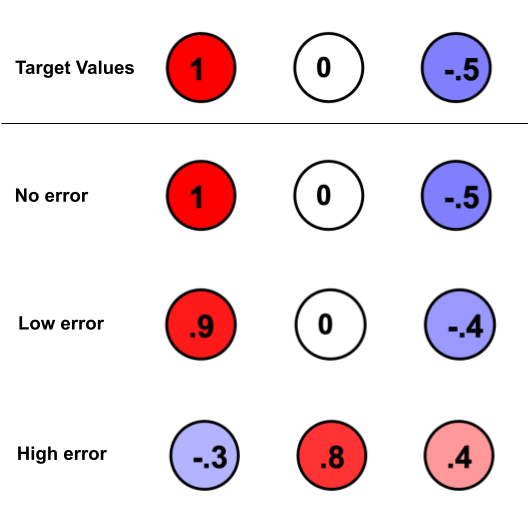
\includegraphics[scale=.3]{./images/ErrorIntuitive.png}
\caption[Jeff Yoshimi.]{Intuitively, error in a neural network corresponds to how close the activations of a set of nodes are to some desired target values. In Simbrain, we can compare how close the actual colors of a pattern of nodes are to some desired pattern.  This is just a first presentation of the idea. It will be made systematic in later chapters.}
\label{intuitiveError}
\end{figure}

The way a neural network is usually trained is by using mathematical techniques to slowly \emph{reduce} error, getting it as close to 0 as possible. This idea is at the heart of the actual techniques used to train neural networks. In practice, numerical errors translate into various kinds of mistake that we can recognize when we use a neural network like ChatGPT.  Perhaps the best-known type of high-level error is a  \glossary{hallucination}, where a language model describes something that does not exist, like a reference to a book that was never written. 

These high-level errors arise from the fact the neural networks use \glossary{generalization}, where properties associated with training data is used to make assumptions about new ``out of sample'' data. Generalizing is usually helpful. It's what makes us so good at recognizing new faces, new voices, and new images, just based on seeing a few.  For example, even if I only hear someone say a few things, I can usually recognize their voice again later when they say new things I've never heard before. If we show a neural network a few hand-written letters, it can often generalize to recognize new letters it has never seen before.  But generalization can also lead to errors, where a neural network makes an assumption based on the data it was trained on, but where that assumption fails to apply to new data that it was not trained on. A book or reference a neural network hallucinates will \emph{sound} like the kind of thing someone would write or publish in some context, but does not exist. These problems exist for humans too. Various forms of cognitive bias and stereotype are examples are based on generalization errors, such as making an assumption about how everyone in Merced is based on just having met 2 or 3 people.

\subsection{Example: The Three Object Detector}

An example that illustrates these ideas is the ``three object detector'',  shown in Fig. \ref{3ObjectClassifier}.\footnote{A video about the three object detector (including information about how to load it) is available at \url{https://youtu.be/yYzUmcPaurI?t=380}. In Simbrain 3 it is a simulation file that must be opened using ``open workspace''. In simbrain 4 it is available from the simulation menu under ``backprop.''} The three object detector has a feed-forward topology with three nodes in the input layer, seven nodes in the hidden layer, and three nodes in the output layer.\footnote{The example is not meant to model the brain directly. It is more abstract:  it classifies inputs in a  brain-\emph{like} way. It takes a pattern of inputs, and transforms those inputs through a network of connections. This is similar to the way information processing occurs in the brain. But it is not a realistic simulation of a brain circuit (as we will see, it is a ``connectionist network'' as opposed to a ``computational neuroscience'' model; it is also similar to how computations are done in engineering applications).} In this example we also see how a network can be linked to a virtual environment. The mouse on the right of figure \ref{3ObjectClassifier} is hooked up to this network. When the mouse is moved around, the activation in the input nodes changes. This simulates the way odor molecules impact the inner lining of the nose, causing sensory neurons to fire at different levels. So the input layer is a kind of simulated nose. 
\begin{figure}[h]
\centering
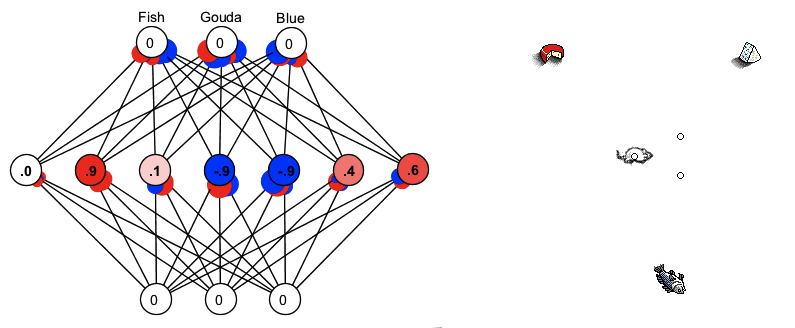
\includegraphics[scale=.4]{./images/3Node_World.png}
\caption[Simbrain screenshot.]{Simple feed-forward network that recognizes three objects.}
\label{3ObjectClassifier}
\end{figure}
% Possibly put in Beer Categorical perception picture here for an example of mixed

Let's first consider its initial performance prior to training.\footnote{In Simbrain 3 the network is loaded pre-trained. To ``untrain'' it  press \texttt{w} and then \texttt{r} to randomize all the weights.} Press play and move the mouse around. (As you do, the weights are not changing). When we move the mouse close to the various objects, it does do anything interesting. It performs in a random way.  We'd like it to react with ``Swiss'' to Swiss cheese, ``Fish'' to fish, and ``Gouda'' to gouda.  So right now, error is high. 

What we can do is train it. We want the network to learn, by updating its weights and other parameters.  Double click on the yellow box above the network to open a training dialog. At the bottom of that dialog, you can see the training data. This describes a few of the associations we'd like this network to perform.  We want it to react to the distributed patterns of ``smell'' at the input layer by classifying what it's smelling at the output layer. We'd also like it to produce a stronger response the closer it is to a given object.  The training data reflect this desired mapping, though not every possible input is included (the network will have to generalize to new inputs it was not trained on). Now press the play button. You can see the error decrease all the way to 0 as the network learns.

Now try running the network again. It now performs the classification task quite well.  As the mouse is moved around to the various objects, it reacts in an appropriate way. So we have trained a network to perform the way we want, by using an automatic procedure to update its weights in a way that reduces error. This shows on a small scale how most neural networks, even massive ones like ChatGPT, are trained.

\subsection{Neural vs. Symbolic Computation}\label{classicalAIComparison}

In the history of cognitive science, one of the earliest debates was between those who thought human information processing was more like what occurs in a classical digital computer--that is, rule-governed manipulation of symbols--and those who thought it was more like what happens in the brain, where patterns of activation are transformed as they propagate through networks of synaptic connections (see section \extref{cog_rev}).\footnote{Of course, neural network simulations are usually run on a traditional computer performing classical computations. But that is a convenient way of implementing the formal structure of a neural network. These implementation can still take advantage of all the special properties of neural networks. Moreover, it is in fact possible to implement neural networks directly on hardware.} We won't go into the details of this debate here, but we will highlight a few prominent differences between the way a digital computer processes information and the way neural networks do, because they help to see what is distinctive about neural networks.

We can use the 3-object detector to illustrate these contrasts. In a classical computer, discrete symbols (comprised of strings of 0s and 1s, or ``bits'') are operated on by rules, in a sequential manner. Bits of information are placed in registers on a computer's central processing unit (CPU), and logical rules in the CPU's instruction set are applied to these bits. Computers are hand-programmed to do useful things. The inside of a CPU and the memory systems on a computer are carefully controlled environments. They do not do well with noisy signals or damage. Computation in a neural network is  different. Neural computation is not based on sequential, rule-based operations on bits; rather, it is based on parallel operations where patterns of node activations are transformed by weight strengths.\footnote{We can often represent this as a transformation of \emph{activation vectors} (lists of activation values) by \emph{weight matrices} (tables representing weight strengths). So, while the basic formalism of classical computation is logic,  the basic formalism of neural networks is \emph{linear algebra}, which we study in chapter \extref{ch_linear_algebra}.}  Neural networks are also more tolerant of noisy signals and damage than digital computers are. Moreover, they are not programmed in the way a computer is, but they are trained in something like the way a human child is.

Let's use the three object detector simulation to consider some of these contrasts in more detail. 

Networks are \emph{trained} via learning rather than being programmed. We show the network what we want it to do, and it learns to do it. In the three object detector, for example, here is (very roughly) what happened: we put the mouse near the fish, and said, ``when you smell something like this, fire your first node.''  Then we did the same thing with the Gouda and blue cheese. Each time we exposed the network to an object, we used the ``backprop'' algorithm (discussed in a chapter \extref{ch_supervised}) to adjust the network's weights. At first, the network made mistakes, but with each exposure to an object, the weights were changed a little, and over time, it got better and better at recognizing cheese, much like how humans and animals gradually get better at doing things with training. This is called supervised learning, since we know the correct output for each input and can tell the network exactly what output it should produce for any given input. The great thing about this is that once we've trained the network on some data, generalization is possible, where it can deal with new data it's never been exposed to before. We can train a network to respond to a bunch of cheese we have available, and on that basis it can recognize new pieces of cheese it's never seen before. This is part of what makes neural networks so valuable, both the one used in your cell phones and also the one that is inside your skull right now helping you read this. After a bit of training and learning, they can be let loose in the world and deal with brand new situations.

% Add discussion of hallucination here, possibly with a glossary entry. Also see new examples in GenAI lectures for 3 object detector and mnist. Distinguish it from other kinds of inference or performance mistakes.

This isn't the only way neural networks can be trained. For example, neural networks can also learn by a system of rewards and punishments (reinforcement learning). They can also learn without any kind of training signal or reinforcement, simply by picking up on the statistical structure of their environment (\glossary{unsupervised learning}).\footnote{Sometimes the weights are hand-crafted, as in the IAC networks discussed in chapter \extref{ch_applications}. But that is the exception that proves the rule. IAC networks are great at illustrating activation dynamics, but are unusual insofar as the weight strengths are not learned from data but are hand-set by a human.}

Second, neural networks emphasize \glossary{parallel processing}. Whereas digital computers normally do things one at a time, in a sequence, neural networks do a lot of things \emph{at the same time}. To see the difference this can make, consider a simple problem: finding which of ten cups has a jelly bean under it. A serial approach would lift each cup up, one at a time, until the jelly bean was found. A parallel approach would lift all ten cups up at once. Neural networks operate like this, processing information in all the nodes, all at once, all the time. This is easy to see  in the three object detector simulation: when you run the simulation and drag the mouse around, the activations of all the nodes will change in parallel based on the new inputs.\footnote{Of course, you run Simbrain on a conventional computer, so that in reality, the neural network is updated in serial. But this is just an artifact for convenience. In our brains, neurons fire in parallel, and large scale simulations of neural networks are also run in parallel (often on massive distributed computing clusters). In fact, all of the advances in the field since 2010 require parallel computation to achieve the required performance.} 

% Do a pass on the footnote below before re-introducing it
%\footnote{Parallel computation is clearly faster. So, why not do everything in parallel? The answer, roughly, is that the whole theory of digital computation assumes a core level of serial processing. To implement a basic algorithm assumes that things happen in a well-ordered fashion. Techniques for parallel computation exist, and are emerging as an important area of computer science, but in those cases tasks are merely broken down into sub-tasks which are each run in serial side-by-side. However not every algorithm is ammenable to this sort of decomposition (many tasks require the full evaulation of some portion of the task before another step in the task can be started) and to make matters worse the physical limitations of computer hardware as it pertains to memory management and allocation prevents even those which are ammenable from achieving peak theoretical performance. With a few (rare) exceptions 8 processing elements (PEs) working on a task in parallel will never complete a task 8x faster than a single PE for these reasons. However this sort of parallelism isn't the same kind of parallelism as what we find in living neural networks. In computer-world we have synchronous, discrete parallelism; in neuro-world we have asynchronous, continuous parallelism. A great many neurons act asynchrnously in parallel each as its own mini-PE sending and receiving signals from sensory inputs and other neurons such that what exactly each neuron is responding to or what its doing can be quite nebulous. The sorts of representation of information that the brain can support are fuzzy and fleeting, but robust. This tends to be excellent for recognizing objects, catching a fly-ball, learning to move, making analogies or being creative, but in general is poorly suited to (for instance) fast, accurate, memory-intensive numerical computation. This fuzziness is perfect for our very fuzzy world, but in the realms math and logic can be prone to mistakes. 

 %Moreover, serial computers are fast these days. For example, the computer I'm writing this on performs several billion operations per second. With numbers like those we can tolerate the processing slow-down due to serial processing.On the other hand, massively parallel processors like the brain are messy, they make mistakes. They are not as good as computers at performing, e.g., complex mathematical computations or looking up names in an index. And they are made of relatively slow materials. Neurons fire at most 200 times per second. They are orders of magnitude slower then the transistors on this computer. In order to solve problems in a reasonable time frame the brain operates in parallel: every neuron is always doing its own thing. The trade-off is in accuracy: the brain is a kind of messy computer, which doesn't always do the same thing twice. But given the wet, biological stuff we're made of, it works well enough.}

% More details on what to do in sim
Third, neural networks experience \glossary{graceful degradation} when they are damaged (this is also called ``fault tolerance''). They are not brittle in the way a digital computer is. You can start deleting the weights of a neural network, and it will still work reasonably well. You can try doing this on the three object detector! In a  similar way, if you lose a few neurons and /or synapses, you will be just fine. Of course, if you lose enough neurons and synapses it, will start to show, but it will happen gradually and  proportionally to the damage. It is in this sense that neural networks degrade ``gracefully.''\footnote{This is related to the fact that they operate in parallel rather than serial. A neural network often has redundant wiring, which can compensate for damage.}  A digital computer, by contrast, is not designed to continue functioning if its components are damaged. Pluck a micro-chip out of the motherboard, or snip a few wires, and there's a good chance your computer will stop working altogether.\footnote{A related point is that neural networks are good at handling \emph{noisy inputs}. Digital computers don't like noisy input: they respond only to clean, precise inputs. Anyone who has worked with computers has some understanding of this. To get through a company's phone tree, you have to enter just the right sequence of numbers--no mistakes allowed!  But show me the same flower ten times, and I will see it as the same flower, even though the input to my brain is changing slightly (the lighting changes, things in my retina change, the whole process is noisy). You can see this in the Simbrain simulation by dragging the mouse around. Notice that even while the inputs change slightly, the network continues to recognize which object it's looking at.}

Fourth, neural networks are well-suited to using \glossary{distributed representation}s, rather than \glossary{localist representation}s (or ``local'' representations). Mental representations (for example, your knowledge of your grandmother) can be thought of in two ways: as being locally stored in one location in the brain, or as being distributed over many locations. A local representation scheme for the brain is sometimes called a ``grandmother cell'' doctrine, because it implies that there is just one neuron in your brain that represents your grandmother. In the context of neural networks, we can say that an object is locally represented by a neuron when activation of that neuron indicates the presence of that object. For example, in figure \ref{localist}, blue cheese is locally represented by the neuron labelled ``Center 5''. When that neuron is activated, the blue cheese is present (here, ``activation'' means having a non-zero, positive activation value).\footnote{Some older types of neural network use local representations (e.g. the IAC networks discussed in chapter \extref{ch_applications}), and we will see that local representations--such as the ``one hot'' representation where only one node in a layer is every active--are sometimes useful. However, the problem with local representations is that you lose some of the virtues above, in particular graceful degradation. If there is just one unit whose activation represents my grandmother, then if I lose that neuron I lose my whole memory of my grandmother. But the empirical evidence suggests that losing a single neuron will not lead to a person's losing an entire memory. So, even if some artificial neural networks use localist schemes to illustrate certain concepts, biological neural networks don't seem to.}

% Sparse (lin alg chap) as intermediate. A few are active, like a smattering of localist nodes.
% Mention polysemanticity and sparse autoencoders. when all the nodes in a network are active it's hard to interpret. One way to deal with this is by converting to localist.


\begin{figure}[h]
\centering
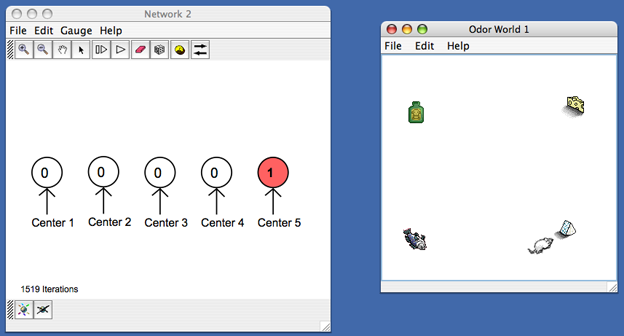
\includegraphics[scale=.3]{./images/Local_Rep.png}
\caption{Localist representation}
\label{localist}
\end{figure}

In contrast, we can say that an object has a distributed representation in a neural network when a particular {\em pattern of activation} over a set of nodes indicates the presence of that object. In figure \ref{distributed},  the bottle of poison has a distributed representation. When the poison is present, a specific pattern of activation $(.1,1,.7,0,.2)$ occurs across the whole set of nodes.   Distributed representations allow multiple representations to exist in a \glossary{superposition} in a layer of nodes.  It has been said that in a network with 100 nodes, up to 100,000 representations can be stored using a superposition of distributed representations \cite{beckmann2025mechanistic}. This is thought to be a key feature of the representations power of modern large language models like ChatGPT.

\begin{figure}[h]
\centering
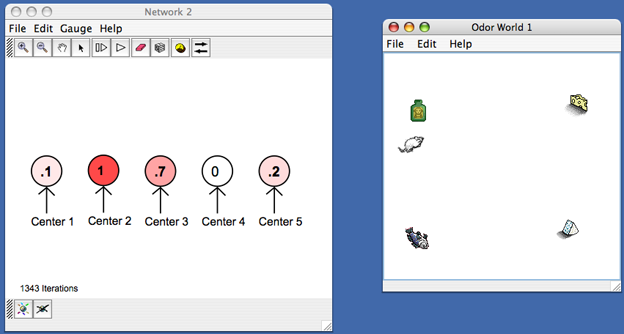
\includegraphics[scale=.3]{./images/Distributed_Rep.png}
\caption{Distributed representation}
\label{distributed}
\end{figure}

For the most part, distributed representations are what one finds in the brain. Generally speaking, brain functions are distributed over many neurons. Although it is harder to think directly about distributed representations than about local representations, a whole conceptual framework has been developed for addressing the problem. In fact, much of the book is about developing a mindset that allows you to think about patterns of activation as points in a space (see in particular chapters \extref{ch_linear_algebra} and \extref{ch_dst}).  From that standpoint, the 3 object detector learns how to detect clusters of points, similar ``smells in smell space.'' 
